\begin{graphicspathcontext}{{./chapters/cps/imgs/},{./chapters/cps/imgs/auto/},\old}

\sidecite{Lee2008CPS}
\begin{frame}{Defining Cyber-Physical Systems}
	\begin{columns}
		\begin{column}{.6\linewidth}
			\begin{definitionblock}{Cyber-Physical Systems (CPS)}
				CPS are \emph{integrations of computation, networking and physical processes}. Embedded computers and networks monitor and control physical processes, with \emph{feedback loops} where physical processes affect computations and vice versa
			\end{definitionblock}
			\begin{block}{Three pillars of CPS}
				\begin{description}
				\item[Physical] real-world dynamics
				\item[Cyber] computation, control, data processing
				\item[Networked] communication, synchronisation
				\end{description}
			\end{block}
		\end{column}
		\begin{column}{.4\linewidth}
			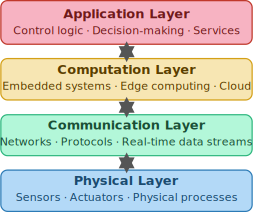
\includegraphics{cps_layers}
		\end{column}
	\end{columns}
\end{frame}

\begin{frame}[t]{CPS Application Domains}
	\begin{columns}
		\begin{column}{.5\linewidth}
			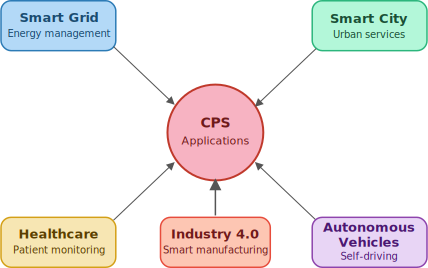
\includegraphics{cps_domains}
		\end{column}
		\begin{column}{.5\linewidth}
			\begin{compactdescription}
			\item[Smart Grid] demand-response, fault isolation
			\item[Smart City] traffic, waste, energy management
			\item[Healthcare] wearable monitors, surgical robots
			\item[Industry 4.0] flexible manufacturing, cobots
			\item[Autonomous Vehicles] perception-control loop
			\end{compactdescription}
			\begin{exampleblock}{Common Challenge}
				All domains require real-time decision-making in open,
				heterogeneous, and uncertain environments.
			\end{exampleblock}
		\end{column}
	\end{columns}
\end{frame}

\end{graphicspathcontext}

\endinput
